\documentclass[UTF8]{ctexart}
\usepackage[]{ctex}
\usepackage{natbib}
\usepackage{graphicx}
\usepackage{enumitem}
\usepackage{setspace}
\bibliographystyle{plain}

\title{LSM-KV 项目报告}
\author{杨景凯 520021910550}
\date{2022年 4月 13日}

\begin{document}

\begin{center}
    \quad \\
    \quad \\
    \kaishu \fontsize{45}{17} 上\quad 海\quad 交\quad 通\quad 大\quad 学
    \vskip 3.5cm
    \heiti \zihao{2} LSM-KV 项目\\
    实验报告
\end{center}
\vskip 3.5cm
\begin{quotation}
    \songti \fontsize{30}{30}
    \doublespacing
    \par\setlength\parindent{12em}
    \quad 
\begin{center}
    学\hspace{0.61cm} 院:\underline{电子信息与电气工程学院}

    学生姓名:\underline{\qquad    \quad \quad 杨景凯    \quad  \quad\qquad }

    学\hspace{0.61cm} 号:\underline{\quad \quad\quad520021910550\quad\quad}
\end{center}
    \centering
    2022年4月13日
\end{quotation}

\clearpage
\tableofcontents

\clearpage
\section{背景介绍}
\subsection{提出背景}
LSM Tree (Log-structured Merge Tree) 是一种可以高性能执行大量写操作的数据结构。它于 1996 年,在 Patrick O'Neil 等人的一篇论文中被提出。\cite{refpdf1}

它的提出是由于考虑到磁盘有如下技术特性:

对磁盘来说,能够最大化的发挥磁盘技术特性的使用方式是:一次性的读取或写入固定大小的一块数据,并尽可能的减少随机寻道这个操作的次数。
LSM-tree充分地利用了这种思想而实现,批次顺序写入大大提高了写性能,因此LSM被设计来提供比传统的B+树或者ISAM更好的写操作吞吐量,通过消去随机的本地更新操作来达到这个目标。\cite{refweb1}
\subsection{项目制作背景}
本次项目制作于学习了跳表和布隆过滤器后。在LSM-KV树中,跳表用于内存结构,布隆过滤器用于优化内存读写速度。

LSM-KV树项目能对跳表和布隆过滤器进行较好的练习,同时也能与B树、B+树、红黑树等对比,加深对内存-磁盘结合的数据结构的理解。同时在项目进行过程中,也能体会到内存和磁盘的读写速度差距。

\section{数据结构和算法概括}
\subsection{跳表}
\subsubsection{基础介绍}
跳表是一个随机化的数据结构,实质就是一种可以进行二分查找的有序链表。在性能上与红黑树或AVL树相似。
\subsubsection{项目应用}
在LSM-KV树项目中,跳表用于在内存中储存数据。它能使得内存中储存的少量数据快速进行更新。
\subsection{布隆过滤器}
\subsubsection{基础介绍}
布隆过滤器实际上是一个很长的二进制向量和一系列随机映射函数。它能够快速查询某元素是否存在。

若一个元素存在,那么它一定不会误报不存在;如果一个元素不存在,可能会误报存在。
\subsubsection{项目应用}
在LSM-KV树项目中,布隆过滤器储存在缓存与文件中,有助于快速判断键值是否存在。

如果在布隆过滤器中不存在,那么该键值一定不存在,可以直接返回未找到;如果在布隆过滤器中存在,那么仍然可能不存在,需要从后续键值中查找。

它的存在能减少许多在元素不存在时的查找时间,从而降低平均查找时延。
\subsection{归并排序}
\subsubsection{基础介绍}
归并排序是建立在归并操作上的一种有效,稳定的排序算法,该算法是采用分治法的一个非常典型的应用。它能将多路已经有序的序列进行合并,成为一个有序的序列。
\subsubsection{项目应用}
在LSM-KV树项目中,归并排序用于两个部分。一个部分是在区间搜索时将搜到的跳表中和每一个sstable中数据进行归并排序;另一个是在compaction时将所选的sstable归并排序生成新的sstable。

\section{测试}
下面将分部分进行测试。

\subsection{性能测试}

\subsubsection{预期结果}

\begin{enumerate}
    \item LSM-KV树有两个优化:
    \begin{enumerate}
        \item 缓存

        缓存使得查询键值是否存在只需要访问内存,不需要访问文件,这极大地缩减了读写磁盘的次数。
        \item 布隆过滤器
        
        布隆过滤器是针对内存进行的优化。能更快地判断键值是否存在。
    \end{enumerate}
    由于以上两个优化措施,使得内存中缓存了SSTable的BloomFilter和索引的查询时延一定小于内存中只缓存了SSTable的索引信息的查询时延,两者一定小于内存中没有缓存SSTable的任何信息的查询时延。
    
    \item Compaction是一个对磁盘进行大量读写的操作,它将小树归并成大树。由于存在对磁盘的大量读写,因此速度会很慢。因此存在Compaction的插入的平均时延一定大于不存在Compaction的插入的平均时延。

    \item 跳表与红黑树性能接近,但是红黑树由于在插入时存在旋转操作,会使得插入时间增加;由于跳表的平衡性不如红黑树,使得跳表查询时间长于红黑树。
\end{enumerate}


\subsubsection{常规分析}
在此部分,我进行的常规分析包括对Get、Put、Delete操作的测试。测试数据中,每对k-v有如下关系:
$$v.length()=k+1$$
测试分为下面两个部分:

\begin{enumerate}
    \item 测试不同数据大小时的操作时延(包括 Get、Put、Delete 操作的时延),为了测试的合理性,我对每个数据大小测量然后计算出平均时延,选择数据量大小分别为1024×64、1024×32、1024×16、1024×1。结果如下表所示:
    \begin{table}[h]
        \centering
        \begin{tabular}{|c|c|c|c|c|}
            \hline
            平均时延(秒/个)&	1024×64&	1024×32&	1024×16&	1024×1\\
            \hline
            PUT&	0.001332&	0.000334&	0.00009&	0.000001\\
            \hline
            GET&	0.000123&	0.000104&	0.000106&	$\approx$0\\
            \hline
            DEL&	0.000128&	0.000106&	0.0001&	    $\approx$0\\
            \hline
        \end{tabular}
        \caption{平均时延测试结果}
    \end{table}
    
    \item 测试不同数据大小时的吞吐(包括 Get、Put、Delete 操作的吞吐),为了测试的合理性,我对每个数据大小测量然后计算出平均吞吐,选择数据量大小分别为1024×64、1024×32、1024×16、1024×1。结果如下表所示:
    \begin{table}[h]
        \centering
        \begin{tabular}{|c|c|c|c|c|}
            \hline
            吞吐量(个/秒)&	1024×64&	1024×32&	1024×16&	1024×1\\
            \hline
            PUT&	750.70&	    2994.27&	11142.41&	837285.36\\
            \hline
            GET&	8160.54&	9587.84&	    9470.70&	3792592.59\\
            \hline
            DEL&	7794.28&	9466.81&	10048.68&	2745308.31\\
            \hline
        \end{tabular}
        \caption{吞吐测试结果}
    \end{table}
\end{enumerate}

\subsubsection{索引缓存与Bloom Filter的效果测试}
在此部分,对比了三种情况GET操作的平均时延,使用的数据量大小为:1024×64。测试数据中,每对k-v有如下关系:
$$v.length()=k+1$$
测试分为下面三个情况:
\begin{enumerate}
    \item 内存中没有缓存SSTable的任何信息,从磁盘中访问SSTable的索引,在找到offset之后读取数据。
    \item 内存中只缓存了SSTable的索引信息,通过二分查找从SSTable的索引中找到offset,并在磁盘中读取对应的值。
    \item 内存中缓存SSTable的Bloom Filter和索引,先通过Bloom Filter判断一个键值是否可能在一个SSTable中,如果存在再利用二分查找,否则直接查看下一个SSTable的索引。
\end{enumerate}
结果如下表所示:
\begin{table}[h]
    \centering
    \begin{tabular}{|c|c|}
        \hline
        数据总量:1024×64 查询总量:1024×32&	平均时延(秒/个)\\
        \hline
        无缓存&	        0.042942\\
        \hline
        无BloomFilter&	0.000062\\
        \hline
        有BloomFilter&	0.000053\\
        \hline
    \end{tabular}
    \caption{索引缓存与Bloom Filter的效果测试结果}
\end{table}

从上结果可以发现,缓存对性能提升巨大,而BloomFilter也能起到一定的提升作用,符合之前的理论分析。
\subsubsection{Compaction的影响}
在此部分,在不断插入数据的情况下,我统计了每秒钟处理的PUT请求个数(即吞吐量),并绘制其随时间变化的折线图。使用的数据量大小为:1024×64。测试数据中,每对k-v有如下关系:
$$v.length()=k+1$$
结果如图所示:
\begin{figure}[h]
    \centering
    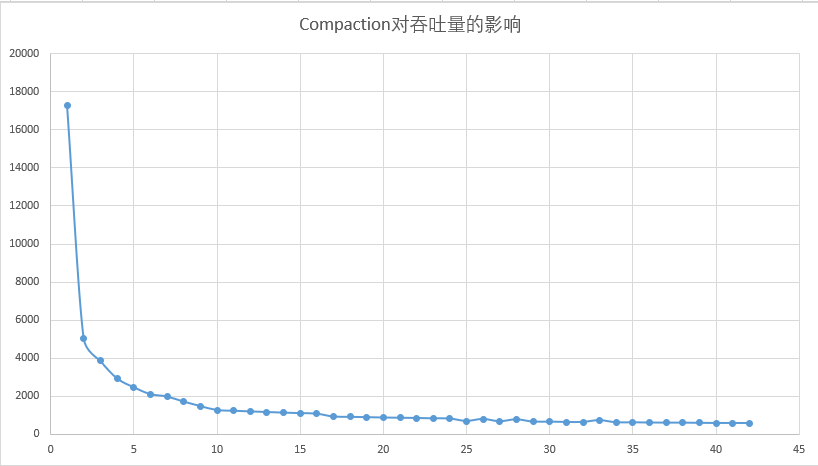
\includegraphics[scale=0.5]{Compaction对吞吐量影响.png}
    \caption{Compaction对吞吐量影响}
\end{figure}

从上结果可以发现,随着数据不断插入,Compaction次数不断增加,吞吐量随时间成指数型下降,在未进行Copmpaction时,平均吞吐量为49871个/秒,两者对比表现出了Compaction对吞吐量的降低程度是巨大的,符合之前的理论分析。
\subsubsection{对比实验}
在此部分,我对比了SkipList和std::map实现MemTable对性能的影响。对比中分别针对PUT、GET、DEL 三个操作进行了测试。使用的数据量大小为:1024×64。测试数据中,每对k-v有如下关系:
$$v.length()=k+1$$
结果如图下表所示:
\begin{table}[h]
    \centering
    \begin{tabular}{|c|c|c|}
        \hline
        数据总量:1024×64&	std::map时延(秒/个)&	SkipList时延(秒/个)\\
        \hline
        PUT&	0.001339&	0.001332\\
        \hline
        GET&	0.000119&	0.000123\\
        \hline
        DEL&	0.000122&	0.000128\\
        \hline
    \end{tabular}
    \caption{对比实验结果}
\end{table}

从上结果可以发现,对于PUT操作来说,SkipList时延较std::Map小,而对于GET、DEL来说,SkipList时延较std::map大,符合之前的理论分析。

因此,对于PUT操作频繁的场景,我们应该使用SkipList做为内存数据结构,而对于查找或删除来说,我们应该使用std::map做为内存数据结构。
\section{结论}
\subsection{项目方面}
本次项目总体来说是成功的,本次我不仅完成了规定的任务,在测试结束后,我还进行了内存泄漏检查,使得程序没有内存泄漏。在项目中,大量使用注释,以及良好的代码风格,使得代码易于复用。
\subsection{结果方面}
本次项目的结果是显然的,许多结论在程序运行中就能明显体会到差别,例如Compaction的影响,缓存的影响等等。结果的得出也是尽如人意的。因此,实验项目结果得出是成功的。
\section{致谢}
\subsection{同学}
在完成项目的过程中,有许多同学对我帮助很大,例如张世昊、彭逸帆。我们一起讨论了各种细节问题、错误原因,使得我本次的项目能够圆满完成,同时也能保有良好的性能。在此表示对这些同学的感谢。
\subsection{开源论坛}
在完成项目的过程中,许多开源论坛、博客帮助我了解了LSM-KV的基础知识,进而使得我能理顺实现思路。在此表示对这些开源论坛和博客的感谢。

\section{其他和建议}
\subsection{针对LSM-KV树的改进}
在 WiscKey (FAST '16) 中,作者提出了一种对 SSD 友好的基于 LSM 树的存储引擎设计。它通过 KV 分离降低了 LSM 树的写放大。 KV 分离就是将大 value 存放在其他地方,并在 LSM 树中存放一个 value pointer (vptr) 指向 value 所在的位置。在 WiscKey 中,这个存放 value 的地方被称为 Value Log (vLog)。由此,LSM 树 compaction 时就不需要重写 value,仅需重新组织 key 的索引。这样一来,就能大大减少写放大,减缓 SSD 的磨损。\cite{refweb2}
\subsection{针对项目代码的改进}
在运行测试后,我们的sstable文件并未删除,而在correctness测试时,并未对LSM-KV树做reset操作。按照LSM-KV树的默认操作,它会读入磁盘中的数据来初始化LSM-KV树,造成测试结果的错误。因此,应该在correctness测试开始前,对LSM-KV树进行reset操作。

此外,我们在讨论中意外地发现。correctness测试中的scan测试组,将list\_ans的插入操作放到循环外,即将LSM-KV树的插入循环与list\_ans的插入循环分离,即可得到巨大的性能提升。分析发现,应该是由于操作系统对程序内存的限制导致的,使得程序来回在虚拟内存与内存上交换数据,造成性能下降。因此,为了测试性能的提升,应该将两个循环分离。

\begin{thebibliography}{99}
    \bibitem{refpdf1}Project.LSM-KV-v1.3.pdf.
    \bibitem{refweb1}https://blog.csdn.net/breakout\_alex/article/details/111305177
    \bibitem{refweb2}https://www.jianshu.com/p/58187ce9d078
\end{thebibliography}

\end{document}
